\documentclass{ximera}

%\addPrintStyle{..}

\begin{document}
	\author{Bart Lambregs, Vincent Gellens}
	\xmtitle{De versnelling}{}
    \xmsource\xmuitleg

	
Een voorwerp versnelt of heeft versnelling wanneer de snelheid verandert in de tijd. Een synoniem voor het woord versnelling is acceleratie, dat het symbool \(\vec{a}\) van deze grootheid verklaart. 
Acceleratie is soms handiger om te gebruiken, dat vermijdt verwarring met het begrip snelheid, wat helemaal niet hetzelfde is!

\(\vec{v}\) = velocity = vitesse = snelheid

\(\vec{a}\) = acceleration = acceleratie = versnelling = snelheids\textbf{verandering}

De vector \(\vec{a}\) grijpt aan op het versnellend voorwerp en wijst in de zin van de ogenblikkelijke bewegings\textbf{verandering}.

\begin{definition}

De gemiddelde versnelling \(\vec{a}\) tussen twee tijdstippen wordt gedefiniëerd als
\[
\vec{a}=\frac{\Delta \vec{v}}{\Delta t}=\frac{\vec{v}_2-\vec{v}_1}{t_2-t_1}
\]
De eenheid van versnelling is meter per seconde, per seconde -- wat meter per seconde in het kwadraat geeft $[a]=\rm\,m/s^2$.

\end{definition}

Als de snelheid van een voorwerp wijzigt, dan wijzigt uiteraard ook de snelheidsvector. Afhankelijk van welk kenmerk van de snelheidsvector (en dus ook van de beweging) verandert, maakt men een onderscheid tussen twee verschillende soorten versnellingen:

\begin{itemize}
    \item Als enkel de \textit{grootte} van de snelheidsvector verandert, spreekt men over een \textbf{tangentiële versnelling \(\vec{a_t}\)}. In dit geval is de versnellingsvector tangentieel of evenwijdig met de snelheidsvector. Dit komt voor bij ééndimensionale bewegingen. Hierbij blijft de richting van de beweging onveranderd.
		\begin{description}
			\item[vb1] Een verticaal omhoog geworpen steen versnelt tangentieel, de bal gaat eerst trager en trager en na het hoogste punt sneller en sneller. Enkel de grootte van de snelheid verandert. De richting niet, want de bal blijft verticaal bewegen.
			\item[vb2] Een auto trekt op een rechte weg op met een versnelling van 3 m/s². Dit wil zeggen dat per seconde de grootte van zijn snelheid met 3 m/s verandert (of in dit geval toeneemt).
		\end{description}
    \item Als enkel de \textit{richting} van de snelheidsvector verandert, spreekt men over een \textbf{normale versnelling \(\vec{a_n}\)}. In dit geval staat de versnellingsvector normaal of loodrecht op de snelheidsvector. Dit komt voor bij tweedimensionale cirkelbewegingen waarbij de grootte van de snelheid onveranderd blijft.
    \item Combinatie van de twee types versnelling is ook mogelijk, bijvoorbeeld bij een schuin geworpen basketbal.
\end{itemize}

\begin{remark}
	De zin van de snelheidsvector kan nooit plots veranderen omdat snelheid een grootheid is die enkel continu in de tijd kan veranderen. De zin van de snelheidsvector kan enkel wijzigen als de grootte van de snelheidsvector vermindert tot nul om dan nadien de tegengestelde zin uit te wijzen. In dit geval gaat het hier dus eveneens over de tangentiële versnelling.
\end{remark}

\begin{image}
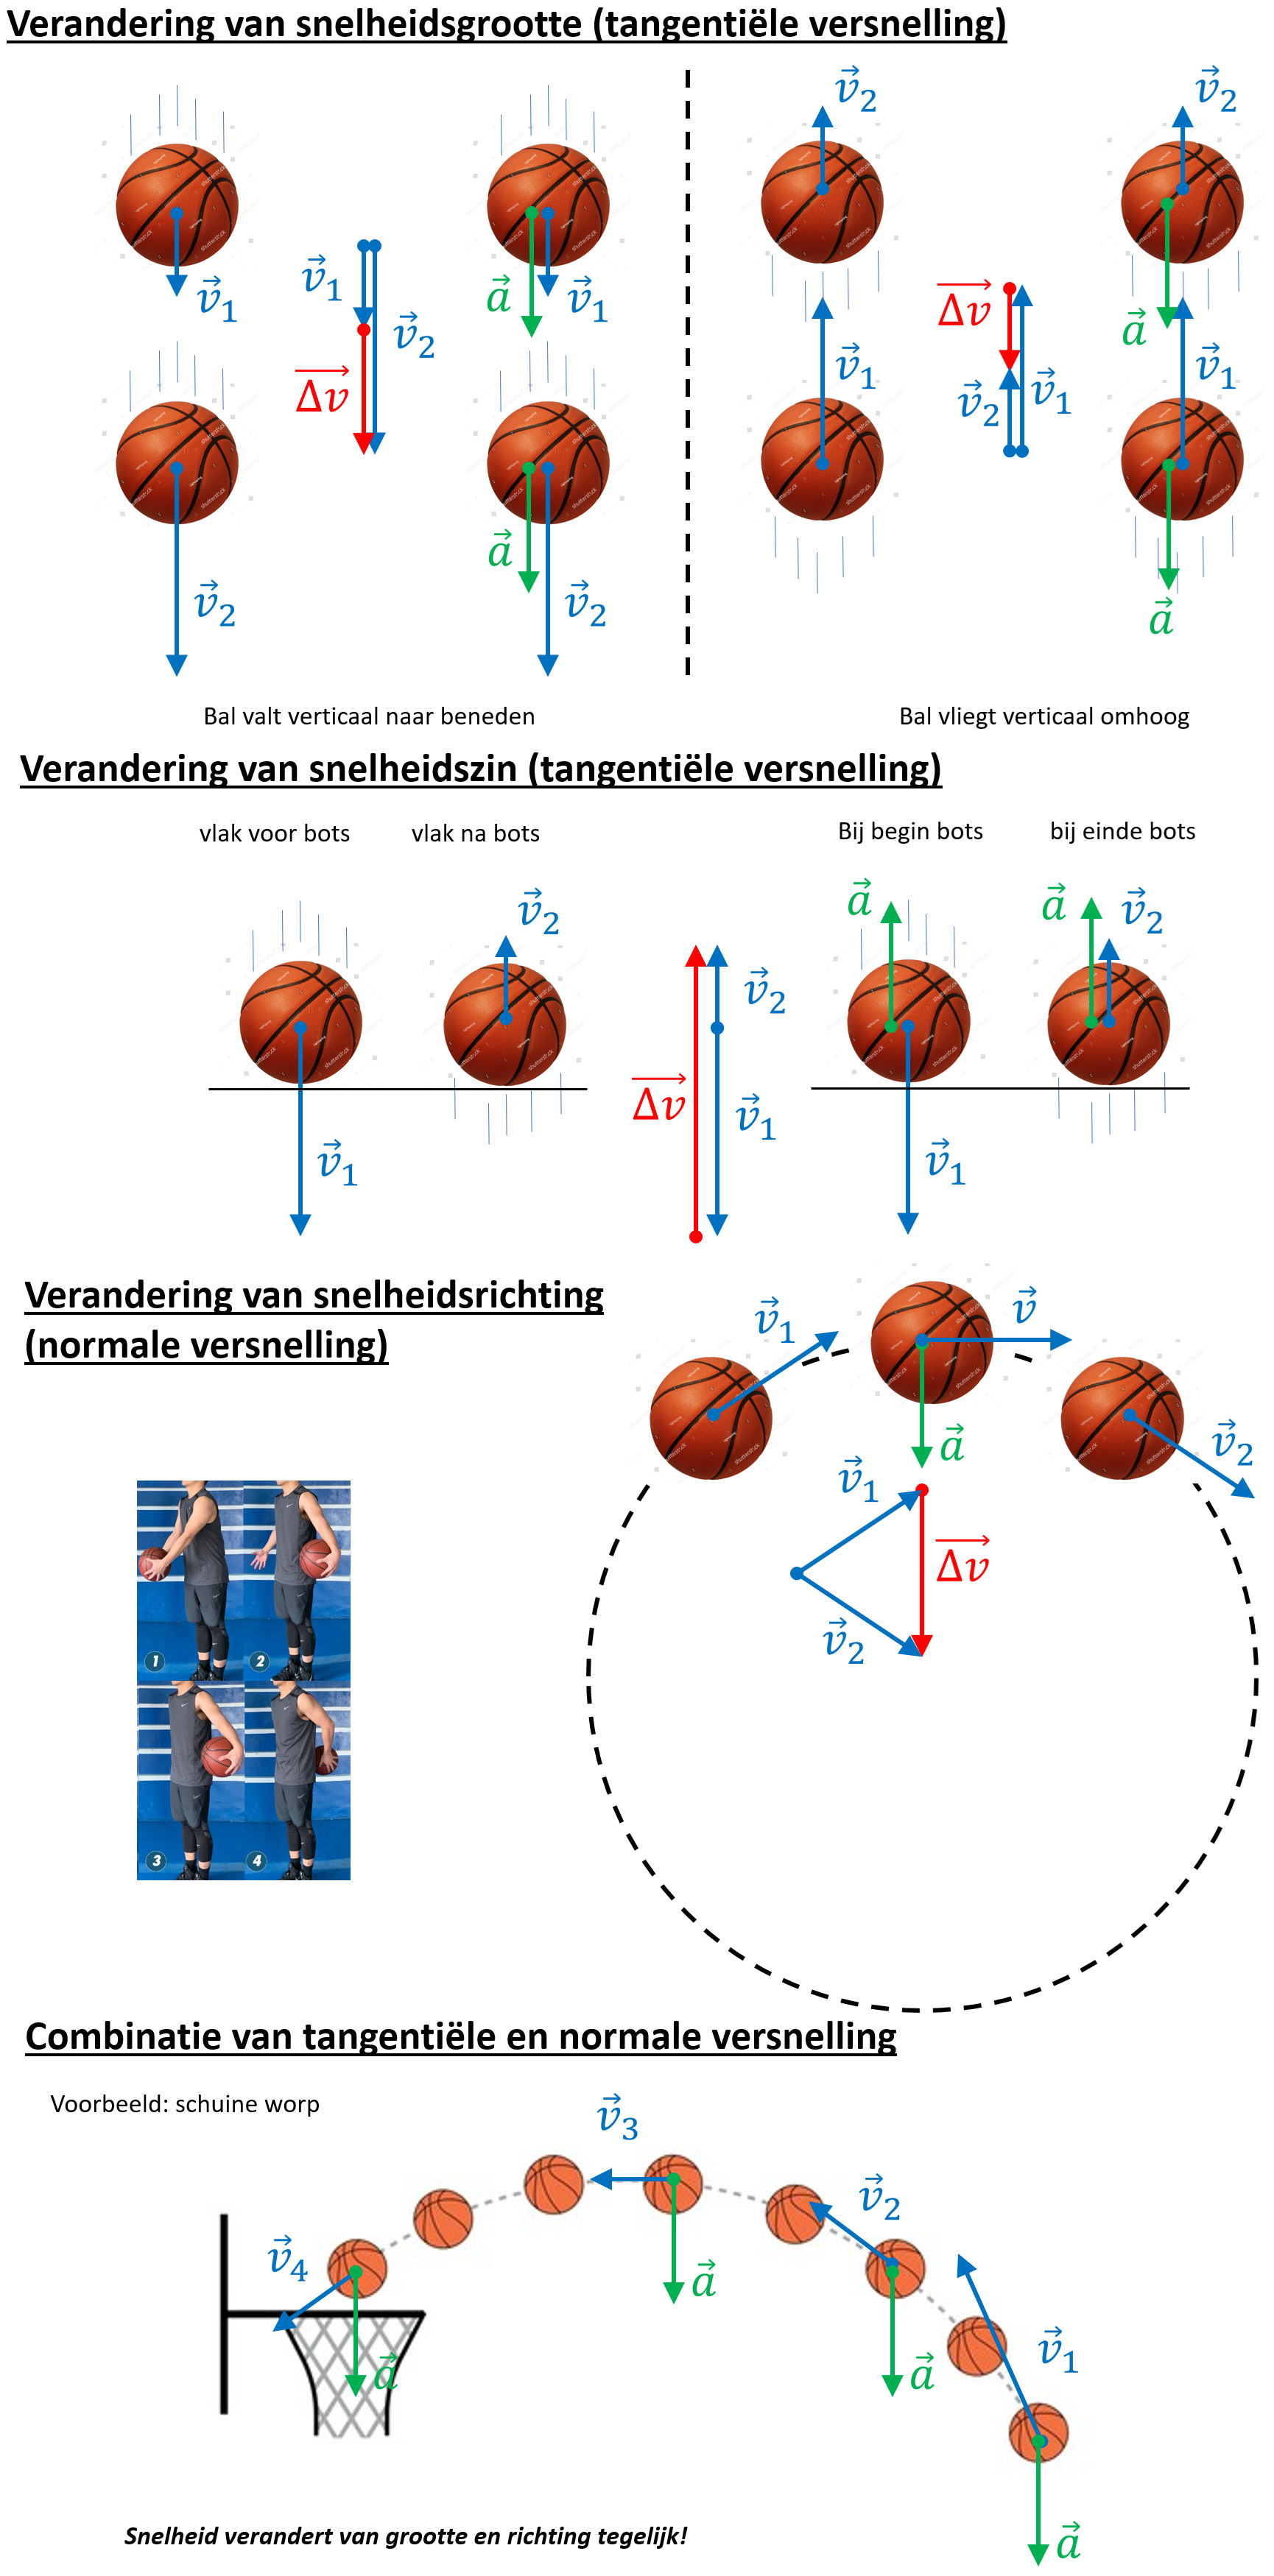
\includegraphics{soortenversnelling}
\end{image}

In al deze voorbeelden lijkt het alsof de versnellingsvector aan de snelheidsvector "trekt".

\subsection*{Gemiddelde (tangentiële) versnelling bij ééndimensionale bewegingen}

\begin{definition}

Bij ééndimensionale bewegingen wordt de gemiddelde versnelling \(\overline{a}\) scalair gedefinieerd als
\[
\overline{a}=\frac{\Delta v}{\Delta t}=\frac{v_2-v_1}{t_2-t_1}
\]
\end{definition}

\begin{denkvraag*}{}
Kan je uitleggen wat de eenheid meter per seconde, per seconde betekent? 
\end{denkvraag*}

\subsection*{Ogenblikkelijke versnelling bij ééndimensionale bewegingen}

De gemiddelde versnelling \(\overline{a}\) geeft de verandering in snelheid \textit{tussen} twee tijdstippen \(t_1\) en \(t_2\).  Om de ogenblikkelijke versnelling \(a\) op één tijdstip \(t\) te bepalen wordt -net zoals bij de ogenblikkelijke snelheid- gebruik gemaakt van de afgeleide. 

\begin{definition}
De ogenblikkelijke snelheid wordt gedefinieerd als de afgeleide van de snelheidsfunctie \(v(t)\):
\[
a=\lim_{t\to t_0}\frac{v(t)-v(t_0)}{t-t_0} = \frac{dv}{dt}=\frac{d^2x}{dt^2}
\]
De notatie met een accent $a(t)=v'(t)$ of $a=v'$ wordt op dezelfde manier als in de wiskunde gebruikt. $a(t)$ is een functie die op elk moment de snelheid geeft. 
\end{definition}

\begin{image}
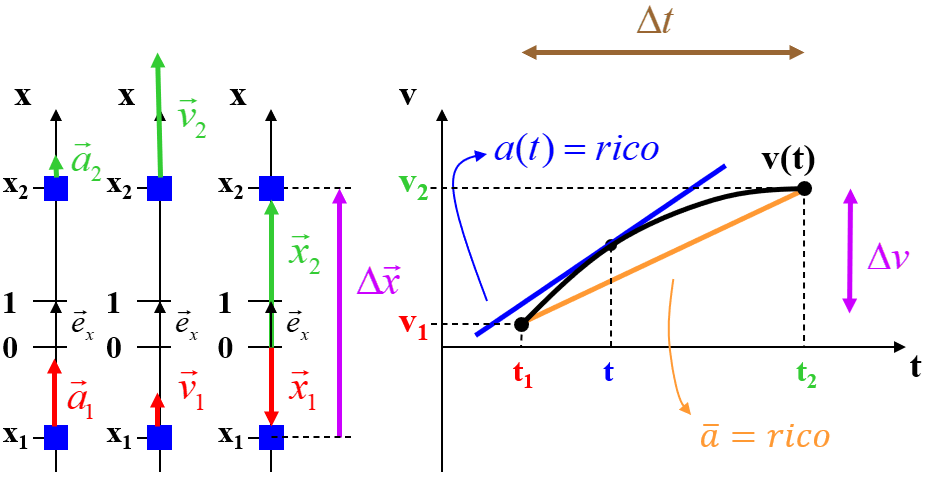
\includegraphics{versnellingmetgrafiek}
\end{image}

In twee dimensies, kan men de versnelling opsplitsen in loodrechte x- en y-componenten. Daarmee kan men analoge redeneringen en gelijkaardige formules maken zoals in het 1D geval.

\begin{image}
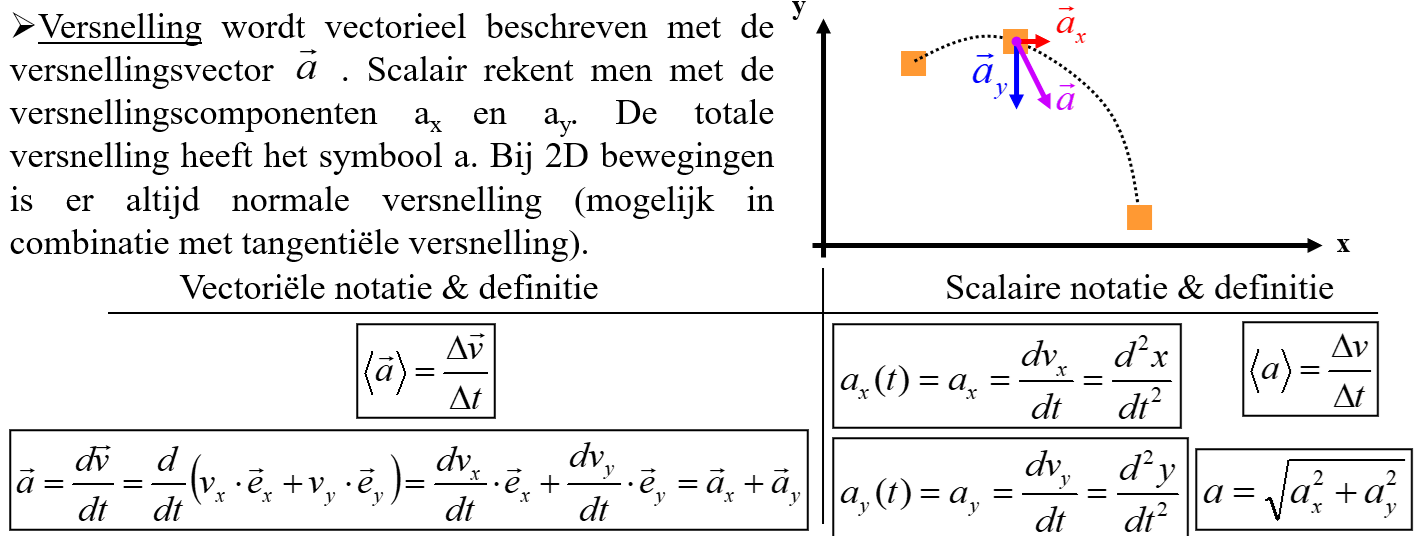
\includegraphics[width=0.8\textwidth]{versnelling2D}

\end{image}

\begin{remark}
	Het begrip versnelling in de fysica heeft niet dezelfde betekenis als hoe het begrip in de volksmond wordt gebruikt.
	\begin{description}
		\item[in de volksmond] 
			\begin{itemize}
				versnelling = vergroten van snelheid

				vertraging = verkleinen van de snelheid

				bocht maken = richtingsverandering van de snelheid
			\end{itemize}
		\item[in de fysica]
			versnelling = verandering van snelheid in eender welk opzicht
	\end{description}

	Fysisch zal men dus nooit spreken over een vertraging. Het vergroten of verkleinen van de snelheid moet bij ééndimensionale bewegingen tot uiting komen in de zin van de versnellingsvector ten op zichte van de zin van de snelheidsvector. Men kan dit ook zien aan het teken van de getalcomponent van de versnelling tegenover die van de snelheid.
	Voor ééndimensionale bewegingen geldt dat als \(\vec{v}\) en \(\vec{a}\) dezelfde zin hebben (of hun getalcomponenten eenzelfde teken hebben) dat de snelheid (in absolute waarde) vergroot. Bij tegengestelde zin (of teken) is er in absolute waarde een verkleining van de snelheid.

\end{remark}

\begin{remark}

	Wagens en fietsen hebben ook versnellingen. Weet dat deze versnellingen nauwelijks iets te maken hebben met het fysisch begrip versnelling. Een auto die in derde versnelling met een constante snelheid van 50 km/h rechtdoor rijdt, versnelt bijvoorbeeld helemaal niet. Zijn versnelling is 0 m/s². Een juistere naam om de standen van de versnellingspook of de ketting weer te geven had eigenlijk “snelheid” geweest omdat de versnelling waarin je rijdt veel meer zegt over welke snelheid je hebt. Kleine versnellingen gebruik je voor kleine snelheden en grote versnellingen voor grote snelheden. Onze Franstalige zuiderburen hebben daar een logischere naam voor, namelijk: “vitesse” (= snelheid). Probeer dus de begrippen snelheid en versnelling niet door elkaar te gooien, want ze hebben een heel andere betekenis! Het is alsof je zou zeggen dat positie en snelheid hetzelfde is!


\end{remark}

\begin{exercise}
Verklaar onderstaande meme. 

\begin{image}
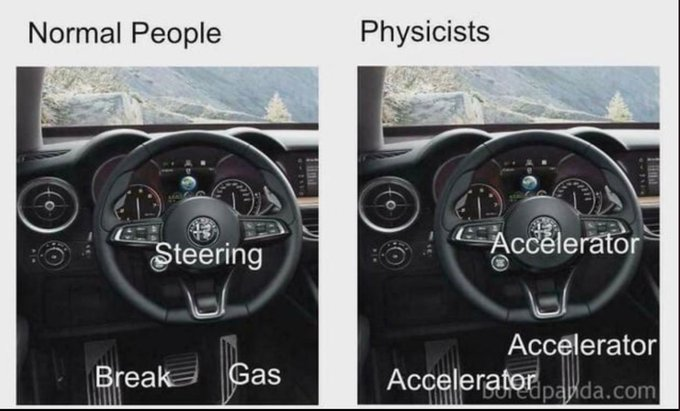
\includegraphics{meme_versnelling}
\end{image}

\end{exercise}
	
\end{document}